\documentclass[tikz,border=2pt]{standalone}
\usepackage{amsmath}
\usepackage{tikz}

\begin{document}
% A partition of [a,b] is any finite increasing list of points starting at a and ending at b;
% the regular subdivision uses n equal subintervals of length (b-a)/n.
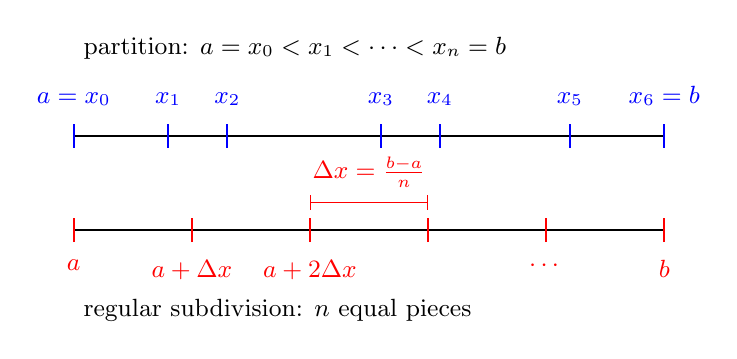
\begin{tikzpicture}[x=1.5cm, every node/.style={font=\small}]
	% general partition
	\node[anchor=south west] at (0,2.05) {partition: $a=x_0<x_1<\dots<x_n=b$};
	\draw[thick] (0,1.2) -- (5,1.2);
	\foreach \x/\l in {0/$a=x_0$, 0.8/$x_1$, 1.3/$x_2$, 2.6/$x_3$, 3.1/$x_4$, 4.2/$x_5$, 5/$x_6=b$} {\draw[blue, thick] (\x,1.05) -- (\x,1.35); \node[blue, above=3pt] at (\x,1.35) {\l};}
	% regular subdivision
	\draw[thick] (0,0) -- (5,0);
	\foreach \i in {0,...,5} {\draw[red, thick] ({\i},-0.15) -- ({\i},0.15);}
	\node[red, below=3pt] at (0,-0.15) {$a$};
	\node[red, below=3pt] at (1,-0.15) {$a+\Delta x$};
	\node[red, below=3pt] at (2,-0.15) {$a+2\Delta x$};
	\node[red, below=3pt] at (4,-0.15) {$\cdots$};
	\node[red, below=3pt] at (5,-0.15) {$b$};
	\draw[red, |-|] (2,0.35) -- (3,0.35);
	\node[red, above=2pt] at (2.5,0.35) {$\Delta x=\tfrac{b-a}{n}$};
	\node[anchor=north west] at (0,-0.75) {regular subdivision: $n$ equal pieces};
\end{tikzpicture}
\end{document}
